\subsection{Auswertung}
Für alle Messungen der $U$-$I$-Kennlinie wird $\sqrt{I-I_0}$ gegen die Gegenspannung $U_\mathrm{G}$ aufgetragen. An die Daten wird eine Anpassungsgerade $\sqrt{I-I_0}(U_\mathrm{G})=aU_\mathrm{G}+b$ angepasst.Für ein kleine Werte von $I-I_0$ wird der aus der linearen Fehlerfortpflanzung resultierende Fehler deutlich größer als die absoluten Fehlerschranken, für diese Werte wurden die Fehlerschranken seperat berechnet. Die Anpassungsgeraden ändern sich dadurch nicht, da ohnehin nur Werte im linearen Bereich beachtet werden. Der Index an der Wellenlänge steht für den Messdurchlauf. Die aus der Anpassung folgenden Werte sind in Tabelle \ref{tab:photoeffekt} zu sehen. Aus den Parametern wird die Grenzspannung über $U_0=b/a$ berechnet.

\begin{table}[h]
  \centering
    \begin{tabular}{c c c c}
      \toprule
      $\lambda/\mathrm{nm}$ & $a\mathrm{V}/ \sqrt{\mathrm{nA}}$ & $b/\sqrt{\mathrm{nA}}$ & $U_0/V$\\
      \midrule
      $365_1$ & $2,08 \pm 0,03 $ &$3,47 \pm 0,01 $ & $1,67 \pm 0,02$\\
      $365_2$ & $2,22 \pm 0,03 $ &$3,52 \pm 0,03  $ & $1,59 \pm 0,02$\\
      $405_1$ & $1,71 \pm 0,01 $ &$2,39 \pm 0,01 $ & $1,39 \pm 0,01$\\
      $405_2$ & $1,86 \pm 0,01 $ &$2,398 \pm 0,009$ & $1,286 \pm 0,009$\\
      $436_1$ & $2,15 \pm 0,08 $ &$2,72 \pm 0,07  $ & $1,26 \pm 0,06  $\\
      $436_2$ & $2,622 \pm 0,009$ &$2,800 \pm 0,004$ & $1,068 \pm 0,004 $\\
      $546_1$ & $3,06 \pm 0,06 $ &$1,789 \pm 0,007$ & $0,58 \pm 0,01$\\
      $546_2$ & $2,4 \pm 0,1  $ &$1,34 \pm 0,03  $ & $0,54 \pm 0,03$\\
      $578_1$ & $2,08 \pm 0,07 $ &$0,992 \pm 0,008$ & $0,48 \pm 0,02$\\
      $578_2$ & $1,81 \pm 0,06 $ &$0,95 \pm 0,01$ & $0,53 \pm 0,02$\\
      \bottomrule
    \end{tabular}
    \caption{Parameter der Anpassungsgeraden}
    \label{tab:photoeffekt}
\end{table}


\begin{figure}[h]
  \centering
  \begin{subfigure}[h]{0.49\textwidth}
    \centering
    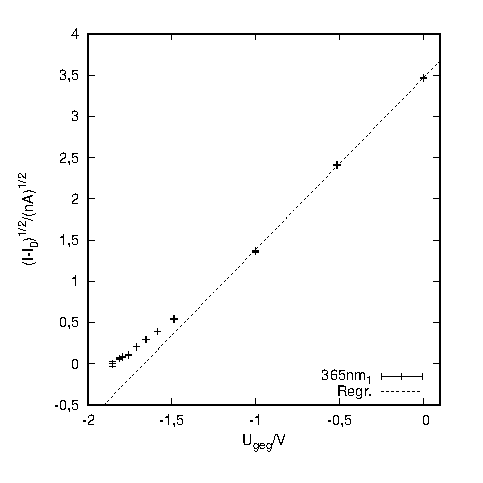
\includegraphics{data/Messung_photoeffekt/365nm_1.eps}
  \end{subfigure}
  \begin{subfigure}[h]{0.49\textwidth}
    \centering
    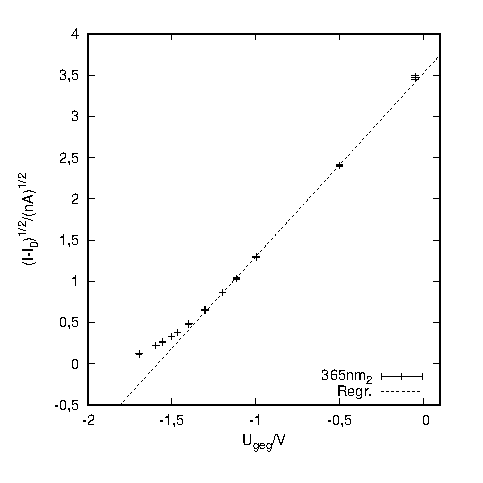
\includegraphics{data/Messung_photoeffekt/365nm_2.eps}
  \end{subfigure}
\end{figure}
\begin{figure}
  \begin{subfigure}[h]{0.49\textwidth}
    \centering
    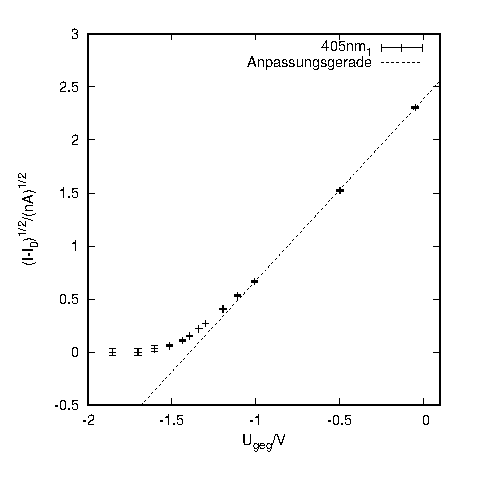
\includegraphics{data/Messung_photoeffekt/405nm_1.eps}
  \end{subfigure}
  \begin{subfigure}[h]{0.49\textwidth}
    \centering
    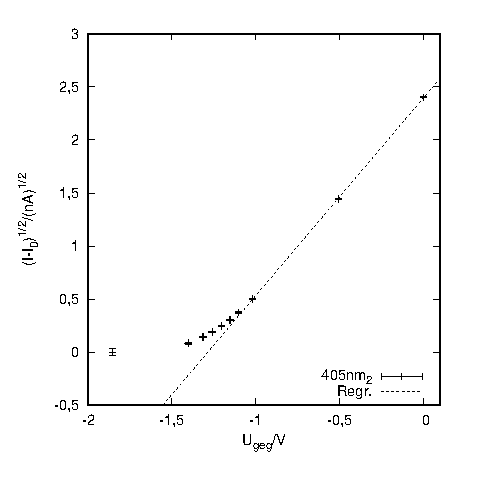
\includegraphics{data/Messung_photoeffekt/405nm_2.eps}
  \end{subfigure}
  \begin{subfigure}[h]{0.49\textwidth}
    \centering
    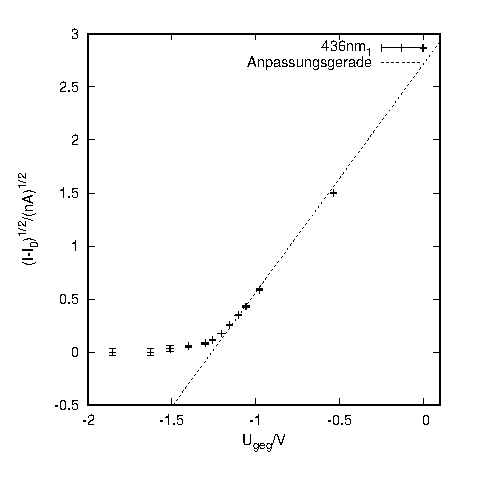
\includegraphics{data/Messung_photoeffekt/436nm_1.eps}
  \end{subfigure}
  \begin{subfigure}[h]{0.49\textwidth}
    \centering
    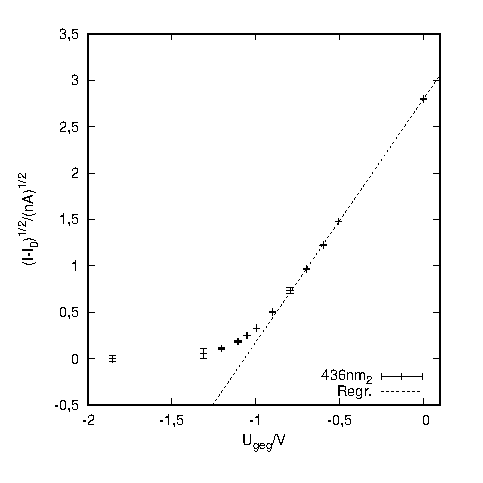
\includegraphics{data/Messung_photoeffekt/436nm_2.eps}
  \end{subfigure}
\end{figure}
\begin{figure}
  \begin{subfigure}[h]{0.49\textwidth}
    \centering
    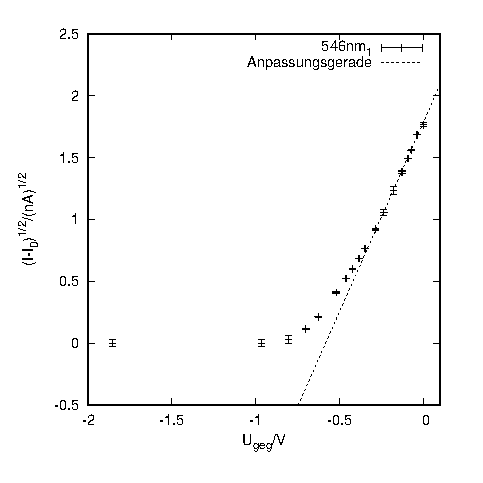
\includegraphics{data/Messung_photoeffekt/546nm_1.eps}
  \end{subfigure}
  \begin{subfigure}[h]{0.49\textwidth}
    \centering
    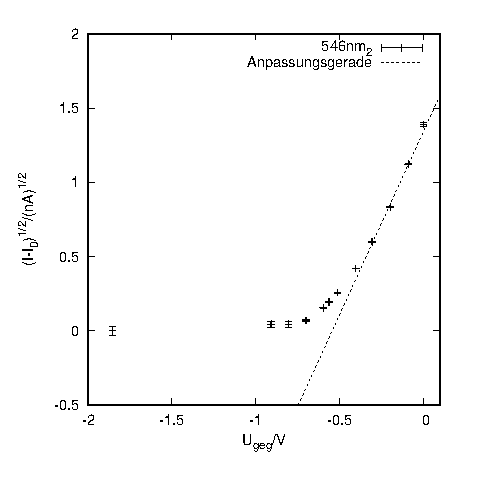
\includegraphics{data/Messung_photoeffekt/546nm_2.eps}
  \end{subfigure}
  \begin{subfigure}[h]{0.49\textwidth}
    \centering
    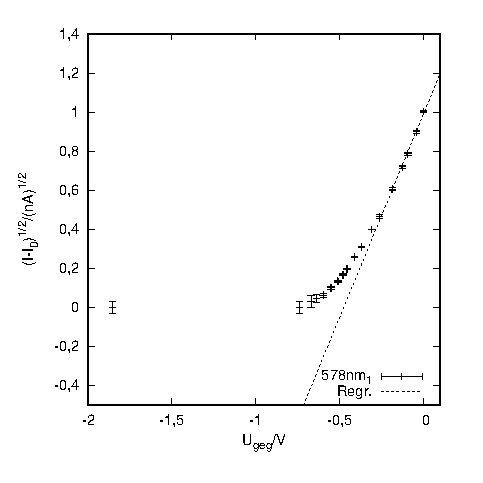
\includegraphics{data/Messung_photoeffekt/578nm_1.eps}
  \end{subfigure}
  \begin{subfigure}[h]{0.49\textwidth}
    \centering
    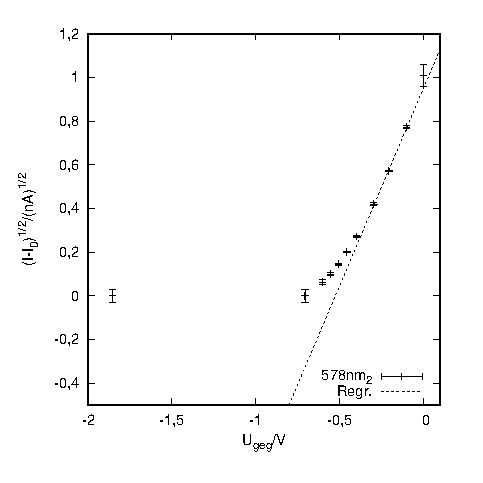
\includegraphics{data/Messung_photoeffekt/578nm_2.eps}
  \end{subfigure}
\end{figure}

Für jede Wellenlänge wird der varianzgewichtete Mittelwert der Grenzspannung $U_0$ berechnet. Dann wird die Grenzspannung gegen die Wellenlänge aufgetragen und eine Gerade $U_0(\nu)=a\nu+b$ angepasst (siehe Abbildung \ref{planck}). Die Parameter sind: 
\begin{align*}
  a&=(3,8 \pm 0,2)10^{-15}\mathrm{Vs}\\  
  b&=(-1,5 \pm 0,2) \mathrm{V}
\end{align*}


Mit Gleichung \ref{eqn:grenzspannung} lassen sich nun das Plancksche Wirkungsquantum und die Austrittsarbeit berechnen:
\begin{align*}
  h&=ea=(6,08 \pm 0,03)10^{-34}\mathrm{Js}\\
  W_\mathrm{A}&=-eb=(1,5 \pm 0,2)\mathrm{eV}
\end{align*}

Die $U$-$I$-Kennlinie bei $365$nm und verringerter Intensität ist in Abbildung \ref{fig:lowintensity} zu sehen. Die Parameter der Anpassungsgerade und die Grenzspannung sind:
\begin{align*}
  a&=(1,32 \pm 0,01)\sqrt{\mathrm{nA}}/\mathrm{V}\\
  b&=(2,07 \pm 0,01)\sqrt{\mathrm{nA}}\\
  U_0&=(1,57 \pm 0,02)\mathrm{V}   
\end{align*}

\begin{figure}[h]
  \centering
  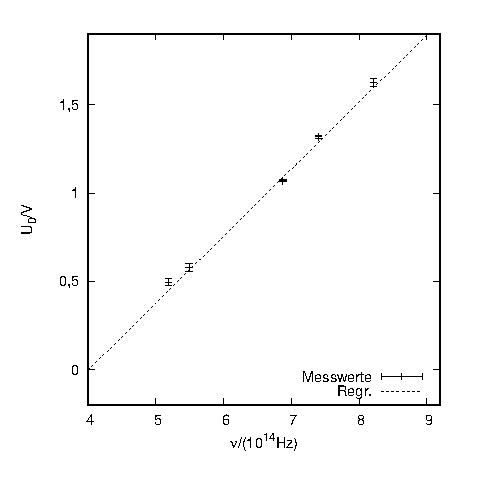
\includegraphics[width=8cm]{data/Messung_photoeffekt/f_u.eps}
  \caption{Grenzspannung und Austrittsarbeit beim Photoeffekt}
  \label{planck}
\end{figure}

\begin{figure}[h]
  \centering
  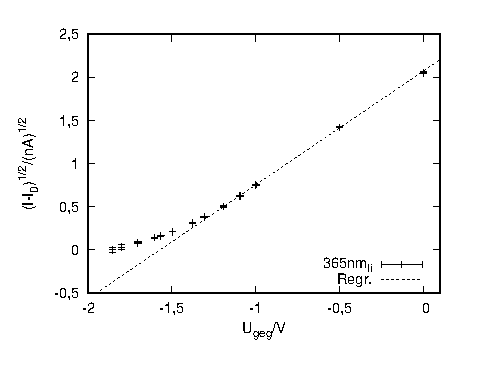
\includegraphics[width=8cm]{data/Messung_photoeffekt/365nm_low_intensity.eps}
  \caption{Kennlinie für 365nm und verringerte Intensität}
  \label{fig:lowintensity}
\end{figure}

\newpage
